
\begin{figure*}[t]
    \centering
    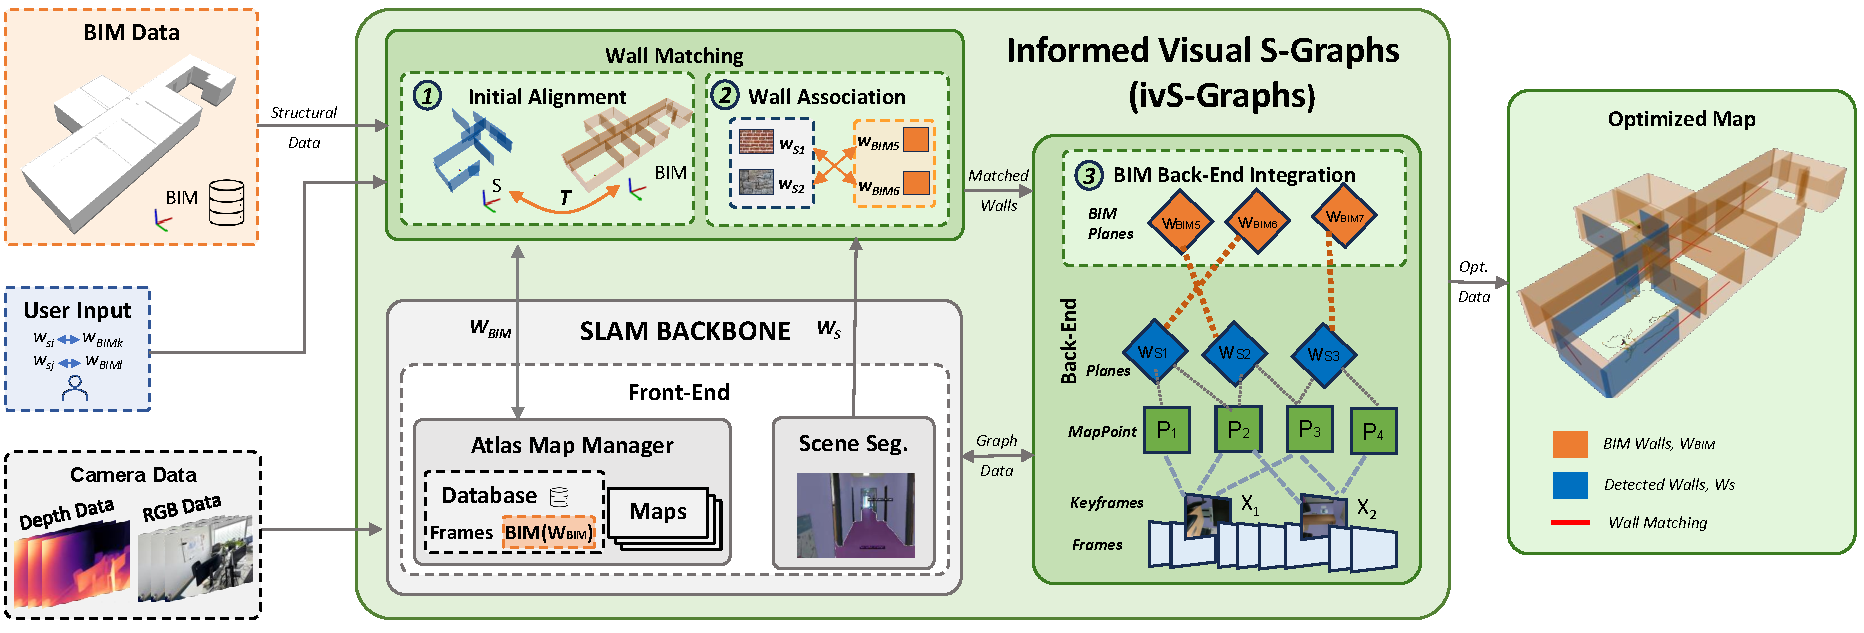
\includegraphics[width=1.0\textwidth]{Figures/RALsys.pdf} % detSys.PNG
% \caption{The system architecture of the proposed system. Modules with a green background are the contributions of the work, while the remaining components provide complementary data.}
% \caption{System architecture of \textit{ivS-Graphs}. The pipeline takes BIM and RGB-D camera data as inputs\add{; BIM walls are extracted offline from the BIM model prior to system operation}. The SLAM backbone front-end processes visual data into keyframes, map points, and wall segments. Our contributions are highlighted in green: (\textbf{1}) initial alignment followed by a (\textbf{2}) continuous wall association and (\textbf{3}) the integration of BIM in the back-end of the system. These establish BIM-to-SLAM correspondences ($\mathbf{W_{\text{BIM}}} \leftrightarrow \mathbf{W_S}$) that are introduced as constraints into the back-end graph. The resulting optimized map (right) aligns the evolving \textit{as-built} structure with the \textit{as-planned} BIM.}
\caption{System architecture of ivS-Graphs. The pipeline takes BIM and RGB-D camera data as inputs and BIM walls are extracted offline from the BIM model. The SLAM backbone front-end processes visual data into keyframes, map points, and wall segments. Our contributions are highlighted in green: (\textbf{1}) initial alignment followed by a (\textbf{2}) continuous wall association and (\textbf{3}) back-end graph optimization incorporating wall-to-wall constraints ($\mathbf{W_{\text{BIM}}} \leftrightarrow \mathbf{W_S}$). This constrains camera drift to produce an optimized as-built map (right) aligned with the design.}
 \label{fig:system_architecture}
% \vspace{-0.3cm}
\end{figure*}

\section{Related Works}
\label{sec_related}


\subsubsection*{\textbf{Visual SLAM in structured environments}}
\textit{ORB-SLAM3}\cite{orb3} provides a widely used feature-based SLAM baseline supporting multiple sensor configurations, and \textit{vS-Graphs}\cite{tourani2025vsgraphs} extends it by integrating structural planes into a factor-graph back-end.
Dense approaches like \textit{BAD-SLAM}~\cite{badslam} offer great geometric detail but often struggle with real-time performance on long construction trajectories. 
More recently, learning-based systems such as DROID-SLAM~\cite{droidslam} and SSF-SLAM~\cite{ssf_slam} have improved robustness through dense bundle adjustment and semantic cues.
However, in construction environments these methods produce drift-affected maps unreliable as an \textit{as-built reference}~\cite{sun2025nothingHilti}.
Since the BIM~\cite{bim} already encodes the expected structural 
layout, it provides a suitable source of architectural priors to 
constrain and correct the SLAM. 

\subsubsection*{\textbf{Global localization with architectural priors}}
A common strategy to integrate prior knowledge, such as BIM or floorplans, in SLAM is to localize the robot within a pre-existing map using particle filters such as Monte Carlo Localization~\cite{dellaert1999monte}. With LiDAR input, this strategy has been extended to use architectural priors for building-scale localization~\cite{blum_precise_2021}.
\add{Further works demonstrate robust pose tracking in CAD drawings~\cite{Boniardi} and semantic BIM-based localization using 2D LiDAR~\cite{Hendrikx}}.
Vision-based methods align monocular RGB detections to 2D floor plans~\cite{zimmerman_constructing_2023} or construct semantic scene graphs conditioned on prebuilt 3D LiDAR maps~\cite{longo2025pixels}. 
While effective for pose estimation, these pipelines localize within a fixed map and do not refine an evolving \textit{as-built} map, often requiring substantial operation for reliable matching.

\subsubsection*{\textbf{Architectural priors in SLAM systems}}
To address these limitations, recent works examine the possibility of coupling BIM with SLAM so that architectural priors directly regularize the trajectory and keep the evolving map consistent with the design. \textit{BIM-SLAM} ~\cite{torres2024bim} integrates BIM into multi-session 3D LiDAR SLAM by seeding a pose-graph from the model, anchoring subsequent sessions to the BIM, and reconstructing new elements not present in the plans. 
Other works combine the \textit{as-built} map and \textit{as-planned} BIM into a joint optimization graph: \textit{iS-Graphs} merges a BIM-derived graph with the online \textit{S-Graph}~\cite{bavle2025s} to enable global localization with room semantics~\cite{isgraphs}, with follow-up work measuring discrepancies between plan and observations~\cite{disgraphs}.
These methods, while benefiting from LiDAR-based high accuracy and $360^\circ$ coverage for room detection, rely on room-level semantics for global localization. This means that in symmetric environments, or when room detection fails or an insufficient number of rooms are observed, these methods cannot establish reliable localization, preventing operation in smaller areas such as a single room.


A few works have extended these ideas to vision-based SLAM. 
For example,~\cite{driftFree} integrates visual SLAM with detailed digital twins to suppress drift; however, \add{this system targets outdoor urban environments and aligns sparse point clouds against a dense photorealistic mesh representing the \textit{as-built} state via ICP. 
This registration is purely geometric, matching points by proximity alone.
Such a dense \textit{as-built} reconstruction must be captured from the environment beforehand, and reflects the clutter and materials that change throughout active construction. Keeping such a prior valid as the site evolves would require its continuous re-capture.}
\add{The \textit{as-planned} BIM available from the design phase offers an alternative: it encodes semantic elements such as walls that do not need to be re-captured as the environment evolves. However, its use in visual SLAM to maintain a drift-bounded \textit{as-built} map remains unexplored, motivating the approach proposed in this work.}
